\documentclass[11pt, a4paper]{article}
\usepackage{fullpage}
\usepackage[USenglish]{babel}
\usepackage{graphicx} 
\usepackage[small,bf,hang]{caption2}
\usepackage{nameref}
\usepackage{hyperref}
\hypersetup{
    colorlinks,
    citecolor=black,
    filecolor=black,
    linkcolor=black,
    urlcolor=black
}

\title{Master Thesis -  Security Aspects in Virtual Networks\\ \textbf{SITREP 14}}
\author{\textbf{Laurent De Wilde} \\ Master of Science in the Applied Computer Science \\ Vrije Universiteit Brussel}
\date{April 8, 2015}

\begin{document}
\maketitle

\section*{Work done}

This is an overview of the work performed in the past two days:
\begin{itemize}
\item Investigated the problem with the broken hard disk. See \nameref{sec:issues}.
\item Protected the virtual disks from mounting and therefore denied access to them.
\end{itemize}
First of all, when a virtual hard disk is in use, that is, when the VM is already started, it is impossible to mount it. Thus the disk gets locked automatically when the VM is started. \\
However, by default, when the VM is not started, it is possible to mount the disk and steal the files on it, as I showed in the previous SITREP. \\ \\
The solution to this is (in my opinion), not to lock but to encrypt the disk using BitLocker. This tool is buillt-in by default in WS2012 R2 (but not enabled by default of course). \\
BitLocker encrypts the hard drive and makes it password-protected so that when an attacker wants to retrieve the data from the disk, (wants to mount it), he first needs to type in a password. When AES 256 bit encryption is used, the process of cracking the password becomes extremely difficult. \\
Also, when the disk is transfered to another Hyper-V server, it is still impossible to mount the disk without knowing the password. Obviously, another password than the Administrator password must be used - since the hacker already knows the (compromised) password of the system. \\ \\
For this purpose, I will demonstrate this using a Windows Server 2012 R2 VM, since BitLocker is only available on the Enterprise or Ultimate versions of Windows 7 and I only have a Professional version of Windows 7 available. \\ \\
First, I have enabled the BitLocker feature and configured it to use 256 bit encryption using group policy.
$\;$ \\ \\
\noindent\begin{minipage}{\textwidth}
    \centering
    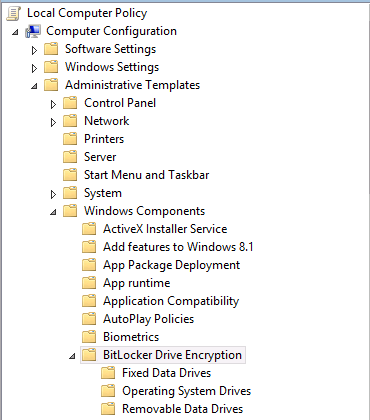
\includegraphics{BitLocker_1.png}
 \captionof{figure}{The BitLocker settings in the group policy of Windows Server 2012 R2.}
\end{minipage}
$\;$ \\ \\
\noindent\begin{minipage}{\textwidth}
    \centering
    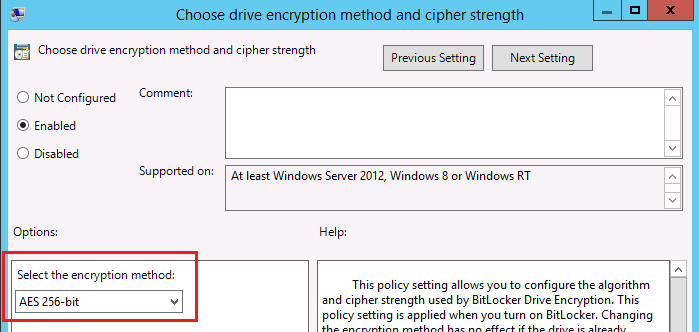
\includegraphics[width=\textwidth]{BitLocker_2.png}
 \captionof{figure}{A 256 bit encryption is chosen for maximum protection.}
\end{minipage}
$\;$ \\ \\
\noindent\begin{minipage}{\textwidth}
    \centering
    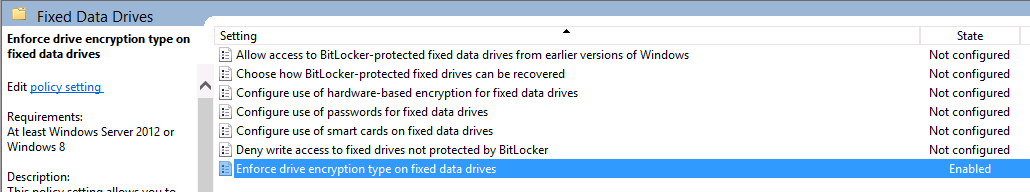
\includegraphics[width=\textwidth]{BitLocker_4.png}
 \captionof{figure}{Also non-system drives can be secured.}
\end{minipage}
$\;$ \\ \\
\noindent\begin{minipage}{\textwidth}
    \centering
    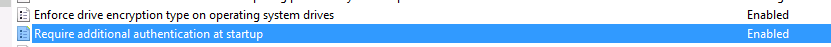
\includegraphics[width=\textwidth]{BitLocker_5.png}
 \captionof{figure}{This setting forces the requirement of entering a password when the VM is started.}
\end{minipage}
$\;$ \\ \\
\noindent\begin{minipage}{\textwidth}
    \centering
    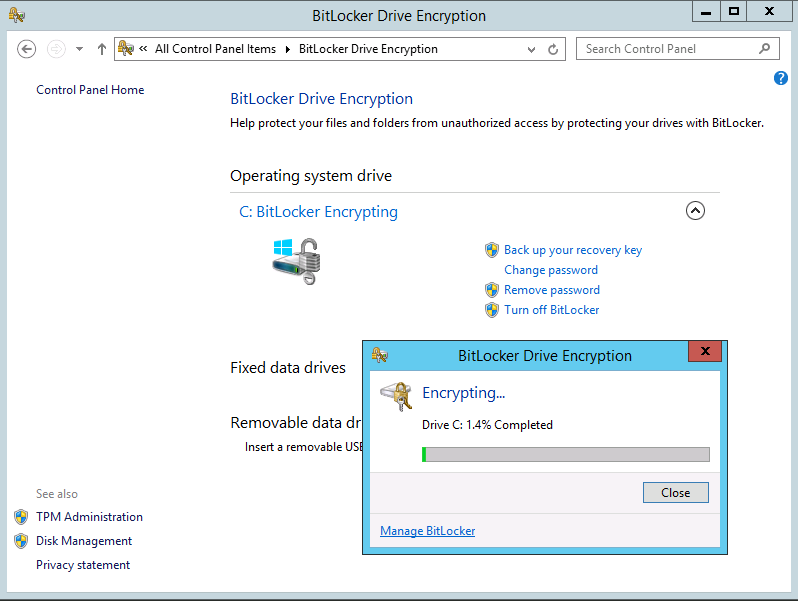
\includegraphics[width=\textwidth]{BitLocker_6.png}
 \captionof{figure}{When the settings are set, the VM is rebooted and ``BitLocker drive encryption'' is selected in the Configuration Panel. Since we want to encrypt the entire VM (and therefore preventing the disk from mounting), the ``C:'' drive is selected.}
\end{minipage}
$\;$ \\ \\
\noindent\begin{minipage}{\textwidth}
    \centering
    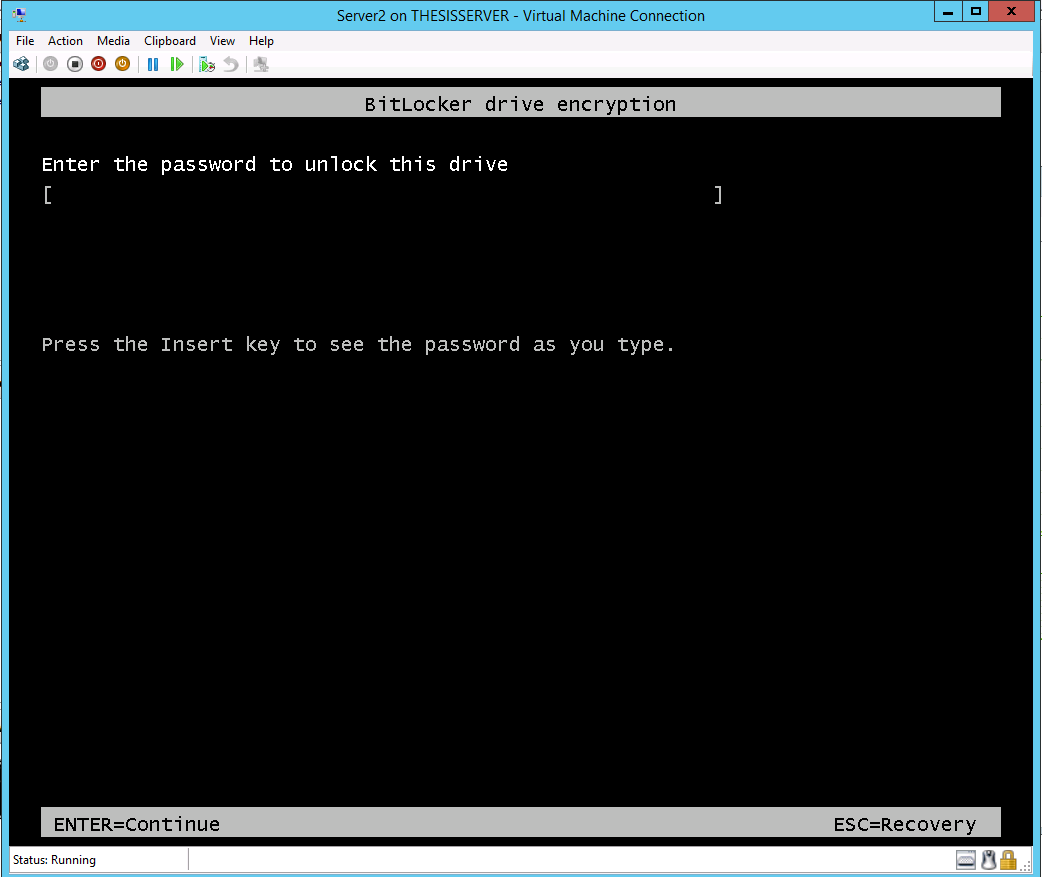
\includegraphics[width=\textwidth]{BitLocker_7.png}
 \captionof{figure}{When the encryption of the system drive has finished, the VM is rebooted and a password is prompted when one wants to boot the VM.}
\end{minipage}
$\;$ \\ \\
\noindent\begin{minipage}{\textwidth}
    \centering
    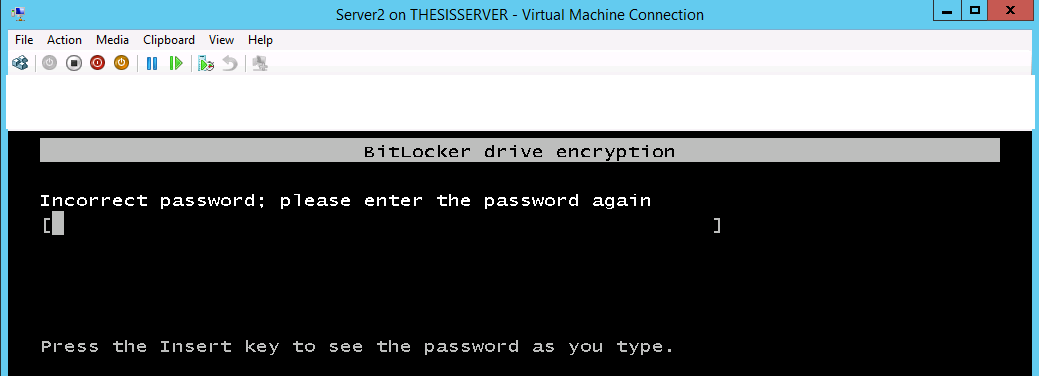
\includegraphics[width=\textwidth]{BitLocker_8.png}
 \captionof{figure}{Without knowing the password, it is impossible to login\ldots . Of course, this prompting for a password at boot time can be disabled in the Group Policy Editor.}
\end{minipage}
$\;$ \\ \\
\noindent\begin{minipage}{\textwidth}
    \centering
    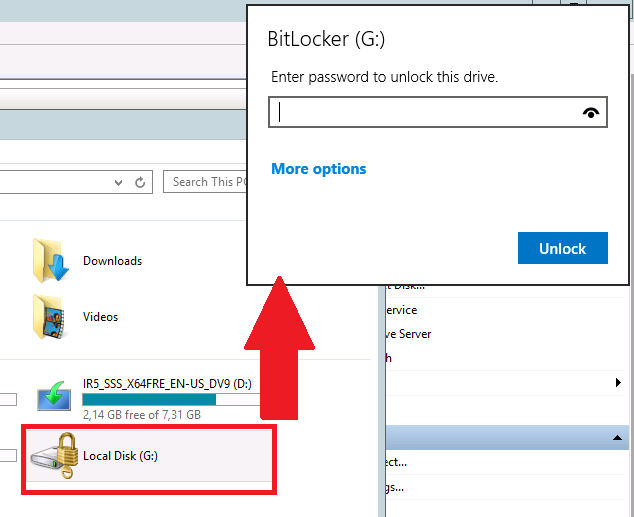
\includegraphics[width=0.85\textwidth]{BitLocker_9.png}
 \captionof{figure}{Now we try to mount the virtual hard drive, but a password is required to do so.}
\end{minipage}
$\;$ \\ \\
\noindent\begin{minipage}{\textwidth}
    \centering
    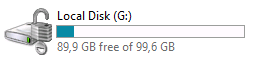
\includegraphics{BitLocker_10.png}
 \captionof{figure}{Only when the correct password is supplied, one is able to access the files on the virtual disk.}
\end{minipage}


\section*{Planning}



\section*{Problems}



\section*{Issues}
\label{sec:issues}
I investigated the problem with the broken hard disk on the 1U pizza server. It turns out that the disk is NOT broken according to the RAID configuration tool. \\
I also swapped the ``broken'' disk bay (the one with the non-blinking LED) with another one (which has a blinking LED) and it turns out that this drive bay is not blinking anymore. So regardless of which drive bay is installed in the slot - the third from right, the LED does not blink. \\
So when the ``broken'' drive bay is installed in the second slot, the LED works fine. \\
The bay, drive and LED are working fine, but apparantly there is something wrong with the connection between the drive bay on the third position and the LED.


\section*{Assistance}


\end{document}